\chapter{EVALUATION}

    \section{Experimental Setup}
    The experiments were executed on a shared cluster with machines running Ubuntu 18.04.2 and having two NVIDIA Tesla V100 GPU cards each. 
    Moreover, they have installations of CUDA 10.1, TensorFlow 1.14, Horovod 0.18.2, OpenMPI 4.0 and NCCL 2.4.8.
    
    For our experimentation we use some publicly available benchmarks created for TensorFlow \cite{tf-benchmark}.
    Each experiment was ran for a fixed number of training epochs and every accuracy we report is based on the test set.
    We use SGD with momentum as an optimizer and we interchange between three different models called Resnet20 \cite{he2015deep}, VGG16 \cite{simonyan2014deep}, and Densenet40 \cite{huang2016densely} all trained on the CIFAR10 \cite{cifar} dataset.
    
    \section{Logging Sampled Information}

    In order to derive information of statistical nature for every experiment, we employ a logging mechanism during the training of the models.
    That is, the bloom filter operators as well as some new, custom operators that we created for this purpose, record frequently information about the compression and decompression of all the gradient vectors.
    In other words, we define a parameter called "verbosity-frequency" which is normally set to 150 and sets all these operators to log information about the actual false positive rates of the bloom filters or the sizes of the messages before and after compression every 150 training steps.
    Then, after the offline processing of this information, we derive statistical results regarding the "Policy Errors Rate" of the experiment, the total number of bits that were sent during all these sampled steps for the communication of the indices or the bloom filter (Initial-Bits, Final-Bits) and so on.
    
    Having said that, we will now explain what every field stands for, in all the following experiments:
    \begin{itemize}
        \item {\bf Initial-Bits} is the total number of bits that are required for the communication of the indices or the values of all the sparsified gradients for all the steps that we selected/sampled without applying any compression method.
        
        \item {\bf Final-Bits} is the total number of bits needed for communicating the same information after applying the compression method that we examine.
        
        \item {\bf Final/Initial} is the ratio: Final-Bits/Initial-Bits. 
        It measures our gain in terms of throughput and we ideally want it to be a lot less than 1.
        
        \item {\bf Policy Errors Rate (PER)} is computed as the total number of times we selected a false positive index over the total number of selections 
        throughout all the steps that we selected/sampled.
    \end{itemize}
    

    
    \newpage
    \section{Indices Compression}
    
    In this section we will provide some experimental results for the bloom filter indices compression method.
    For all of our experiments we used the lossless run length encoding as a baseline and unless specified otherwise, all the bloom filter compression experiments were tuned to be based on the Top-r sparsification method with a compress ratio of $0.01$.
    
    \subsection{Comparison Between Different Policies}

    \begin{figure}[h]
    \centering
    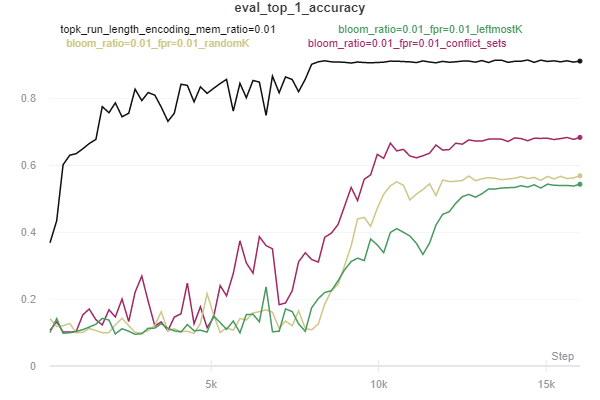
\includegraphics[width=1\textwidth]{figures/resnet20-policies.png}
    \caption{Resnet20, Leftmost-r, Random-r, Conflict Sets}
    \label{policies-comparison}
    \end{figure}
    
    \vspace{1cm}

    As we previously mentioned, training seems to be sensitive to the re-construction errors induced by the occurrence of bloom filter false positive responses.
    Without the algorithmic modification of the "False Positive Aware Compression" none of the models seemed to reach the baseline's test set accuracy.
    In figure \ref{policies-comparison} and table \ref{table:1}, we demonstrate how the selection of different policies affects the model's ability to learn by keeping the compress and false positive ratios fixed and alternating between the policies we discussed in a previous chapter.
    
    We can see in table \ref{table:1} that "Random-r" is marginally better than "Leftmost-r", however, both are significantly worse than the "Conflict Sets" policy which works in a more elaborate way and selects more correct indices. 
    None of the above policies though, can achieve an accuracy as high as the baseline method.
    
    Not that, in figure \ref{policies-comparison}, we have not applied the "memory compensation" feature for any of the bloom filter experiments.
    If we enable this without treating the re-construction errors then those will be catastrophic for training.
    When we compute the difference (delta) between each tensor and its re-constructed version those errors will start to accumulate and affect not only the current step but future steps as well.

    \begin{table}[h!]
    \footnotesize
     \centering
    \begin{tabular}{ |p{3cm}||p{1cm}|p{1cm}|p{1.3cm}|p{1.5cm}|}
    \hline
    \multicolumn{5}{|c|}{\textbf{\footnotesize Resnet20, compress\_ratio=0.01, Top-r}} \\
    \hline
    \rule{0pt}{3ex}
    	Method & Policy & FPR  & PER & Accuracy\\
    \hline
    \rule{0pt}{3ex}
    \multirow{3}{*}{\textbf{Bloom}}
    & L    &0.01     &56.9\%   &48.91\%\\
    & R    &0.01     &51.82\%   &54.41\%\\
    & CS   &0.01     &18.72\%   &68.42\%\\
    \hline
    \rule{0pt}{3ex}
    \textbf{RLE}    & - & - &0   &91.27\%\\
    \hline
    \end{tabular}
    \caption{Bloom Filter Compression: Leftmost-r, Random-r, Conflict Sets}
    
    This experiment was executed on 4 nodes having the aforementioned specifications.
    The FPR is specified by the user and affects the size of the bloom filter as well 
    the number of hash functions.
    \label{table:1}
    \end{table}
    
    \subsection{False Positive Aware Compression}

    \subsubsection{Top-r / Varying FPR}
    In figure \ref{fpa-compression}, we have re-trained resnet20 on cifar10, but this time we have applied the algorithmic modification of the "False Positive Aware Compression". 
    Now, while the selection of false positive indices still occurs, we do not have re-construction errors as every index will be paired with its correct, original value either it is a true positive index or not.
    
    In this experiment, we alternate between different false positive ratios in order to control the size of the bloom filter and thus, the throughput.
    Note that, in our framework, the user implicitly controls the bloom filter size and number of hash functions with the help of the FPR.
    This is achieved by using the mathematical formulas that were described in an earlier section and letting them derive those two parameters as a relation of the false positive rate that is given as input by the user.
    As the FPR gradually increases, the bloom filter size decreases.
    While this creates a spike in the false positive responses, the number of bits required to represent the indices is significantly reduced.
    Now, the more false positives we have the more we "deviate" from the Top-r sparsification method since we sacrifice some of the Top-r values by replacing them with others.
    
    This trade-off demonstrates the flexibility of the bloom filter approach compared to the "Run Length Encoding" baseline. 
    The user can substantially control the size of the message by setting the FPR accordingly. 
    This way they can choose between better throughput or better accuracy or they can simply come up with a tuning that satisfies both in an accepted level.
    Note that, the more we deviate from the Top-r sparsification method the more we degrade to the Random-r method which, in most cases, is not as good in terms of accuracy as the former one \cite{10754/662495}.
    Run Length Encoding, on the other hand, cannot be tuned in a similar way, since it is not a lossless compression method.
    
    Also, having treated the re-construction errors, we can now enable the "memory compensation" feature for the bloom filter experiments, contrary to the previous set of examples. 
    This enables the accuracy to increase and allows the False Positive Aware Compressor to compete with the baseline.
    
    \newpage
    
    %%%%%%%%%%%%%%%%%%%%%%%%%%%%% RESNET20 %%%%%%%%%%%%%%%%%%%%%%%%%%%%%%%%%%%%%%%%%%
    \begin{figure}[h]
    \centering
    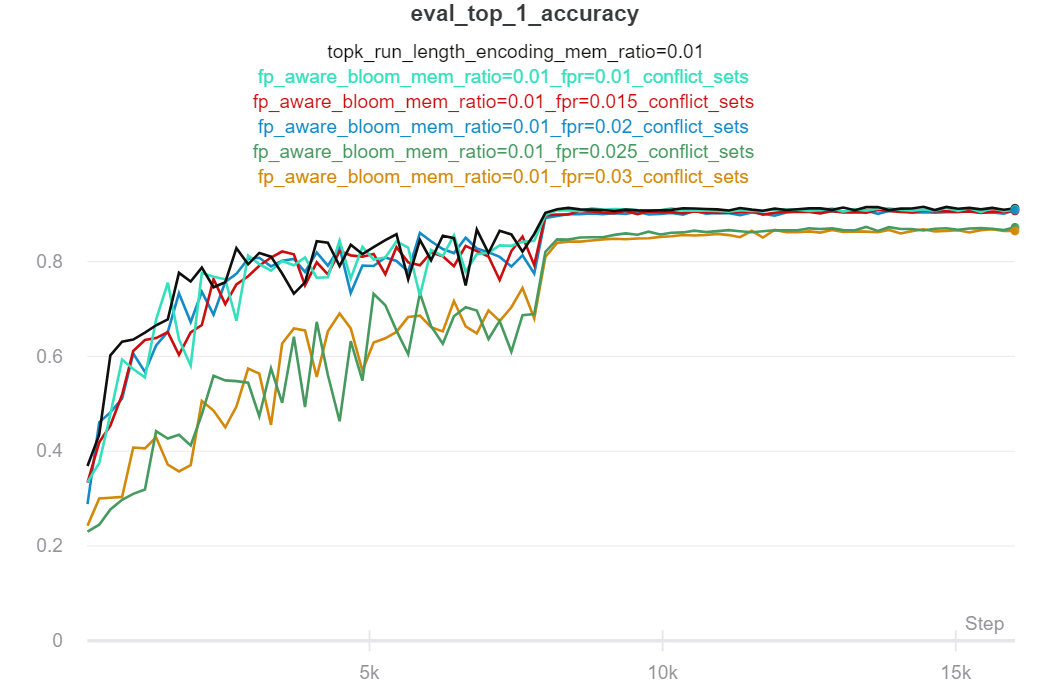
\includegraphics[width=1\textwidth]{figures/fp_aware_resnet20.png}
    \caption{Resnet20, False-Positive-Aware Bloom Filter Compression}
    \label{fpa-compression}
    \end{figure}

    \vspace{1cm}

    Resnet20 has 269,467 training parameters and 51 gradient vectors.
    It was trained on 4 nodes, on the CIFAR-10 dataset for 328 epochs and with no compression at all, it reaches a \textasciitilde91\% accuracy.
    We observe that the False Positive Aware compressor reaches the baseline's accuracy for FPRs up to 0.02 and it starts declining for higher values.
    We can see that as the FPR increases so does the Policy Errors Rate which causes the decline in accuracy.
    
    \vspace{1cm}

    \begin{table}[h!]
    \footnotesize
     \centering
    \begin{tabular}{ |p{3cm}||p{1cm}|p{1cm}|p{2cm}|p{1.6cm}|p{1.6cm}|p{1.3cm}|p{1.5cm}|}
    \hline
    \multicolumn{8}{|c|}{\textbf{\footnotesize Resnet20, compress\_ratio=0.01, Top-r, memory\_compensation}} \\
    \hline
    \rule{0pt}{3ex}
    	Method & Policy & FPR  &Initial-Bits &Final-Bits &Final/Initial & PER & Accuracy\\
    \hline
    \rule{0pt}{3ex}
    \multirow{6}{*}{\textbf{Fp-Aware Bloom}}
    & CS   &0.01     &   28867209 &   2817096 &   9.759\%  &19.25\%   &91.01\%\\
    & CS   &0.015    &   28867209 &   2585120 &   8.955\%  &33.97\%   &90.7\%\\
    & CS   &0.02     &   28867209 &   2409640 &   8.347\%  &44.68\%   &90.88\%\\
    & CS   &0.025    &   28867209 &   2241864 &   7.766\%  &55.32\%   &87.24\%\\
    & CS   &0.03     &   28867209 &   2128016 &   7.372\%  &63.53\%   &86.47\%\\
    \hline
    \rule{0pt}{3ex}
    \textbf{RLE}    & - & - & 28867209 & 2749080 & 9.523\%  &0   &91.27\%\\
    \hline
    \end{tabular}
    \caption{Resnet20: RLE vs FP Aware Bloom Filter Compression}
    Initial-Bits and Final-Bits refer to the indices and not the whole message. 
    \label{table:2}
    \end{table}
    %%%%%%%%%%%%%%%%%%%%%%%%%%%%%%%%%%%%%%%%%%%%%%%%%%%%%%%%%%%%%%%%%%%%%%%%%%%%%%%
    

    %%%%%%%%%%%%%%%%%%%%%%%%%%%%%% DENSENET40 %%%%%%%%%%%%%%%%%%%%%%%%%%%%%%%%%%%%%
    \newpage
    
    In figure \ref{fpa-densenet} and table \ref{table:3},
    we provide the results of similar experiments for the Densenet40-K12 model.

    \begin{figure}[h]
    \centering
    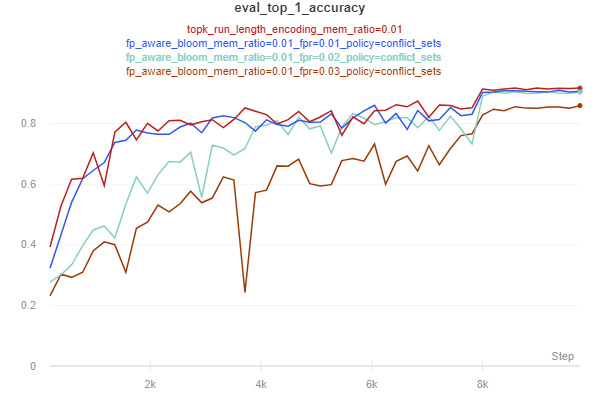
\includegraphics[width=1\textwidth]{thesis/figures/densenet40-bloom.png}
    \caption{Densenet40, False-Positive-Aware Bloom Filter Compression}
    \label{fpa-densenet}
    \end{figure}

    \vspace{1cm}

    Densenet40-K12 has 357,491 training parameters and 158 gradient vectors.
    It was trained on 4 nodes, on the CIFAR-10 dataset for 328 epochs and with no compression at all, it reaches a \textasciitilde92\% accuracy.
    
    \vspace{1cm}

    \begin{table}[h!]
    \footnotesize
     \centering
    \begin{tabular}{ |p{3cm}||p{1cm}|p{1cm}|p{2cm}|p{1.6cm}|p{1.6cm}|p{1.3cm}|p{1.5cm}|}
    \hline
    \multicolumn{8}{|c|}{\textbf{\footnotesize Densenet40, compress\_ratio=0.01, Top-r, memory\_compensation}} \\
    \hline
    \rule{0pt}{3ex}
    	Method & Policy & FPR  &Initial-Bits &Final-Bits &Final/Initial & PER & Accuracy\\
    \hline
    \rule{0pt}{3ex}
    \multirow{4}{*}{\textbf{Fp-Aware Bloom}}
    & CS   &0.01     &   23594406 &   2331648 &   9.882\%  &18.66\%   &90.68\%\\
    & CS   &0.02     &   23594406 &   1997424 &   8.466\%  &45.36\%   &90.4\%\\
    & CS   &0.03     &   23594406 &   1745568 &   7.398\%  &62.89\%   &85.93\%\\
    \hline
    \rule{0pt}{3ex}
    \textbf{RLE}    & - & - & 23594406 & 2391232 & 10.13\%  &0   &91.74\%\\
    \hline
    \end{tabular}
    \caption{Densenet40-K12: RLE vs FP Aware Bloom Filter Compression}
    Initial-Bits and Final-Bits refer to the indices and not the whole message. 
    \label{table:3}
    \end{table}
    %%%%%%%%%%%%%%%%%%%%%%%%%%%%%%%%%%%%%%%%%%%%%%%%%%%%%%%%%%%%%%%%%%%%%%%%%%%%%%%


    %%%%%%%%%%%%%%%%%%%%%%%%%%%%%%%% VGG16 %%%%%%%%%%%%%%%%%%%%%%%%%%%%%%%%%%%%%%%
    \newpage
    
    In figure \ref{fpa-vgg16} and table \ref{table:4}, 
    we provide the results of similar experiments for the VGG16 model.
    
    \begin{figure}[h]
    \centering
    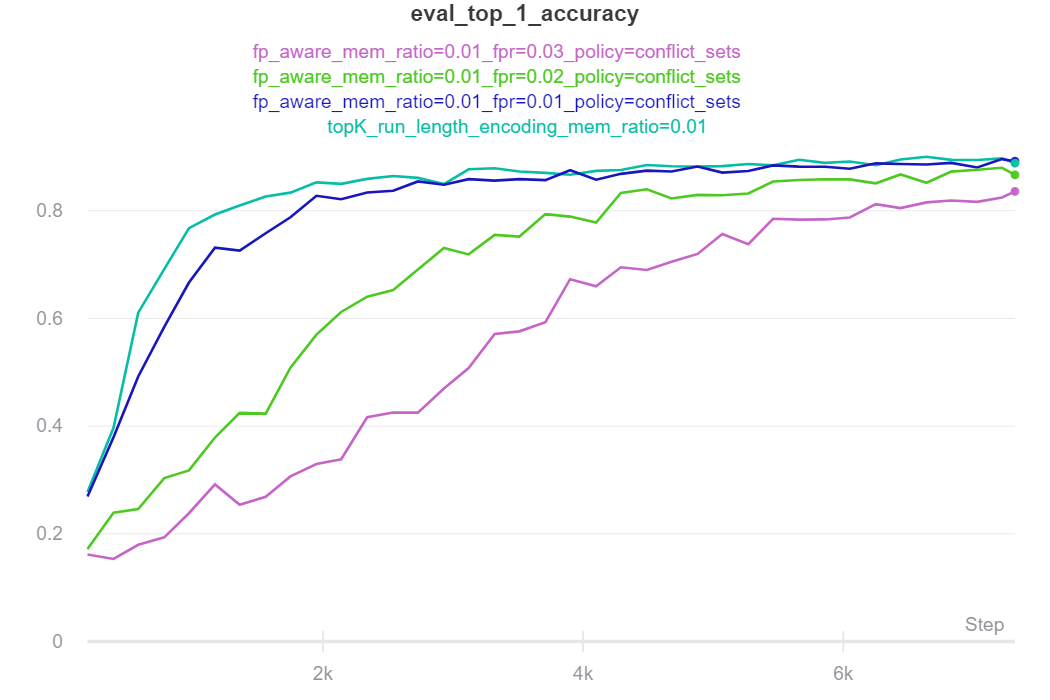
\includegraphics[width=1\textwidth]{thesis/figures/vgg16-bloom.png}
    \caption{VGG16, False-Positive-Aware Bloom Filter Compression}
    \label{fpa-vgg16}
    \end{figure}
    
    \vspace{1cm}

    VGG16 is a huge model having 14,982,987 training parameters and 30 gradient vectors.
    It was trained on 4 nodes, on the CIFAR-10 dataset for 200 epochs and with no compression at all, it reaches an \textasciitilde89\% accuracy.
    
    \vspace{1cm}

    \begin{table}[h!]
    \footnotesize
     \centering
    \begin{tabular}{ |p{3cm}||p{1cm}|p{1cm}|p{2cm}|p{1.6cm}|p{1.6cm}|p{1.3cm}|p{1.5cm}|}
    \hline
    \multicolumn{8}{|c|}{\textbf{\footnotesize VGG16, compress\_ratio=0.01, Top-r, memory\_compensation}} \\
    \hline
    \rule{0pt}{3ex}
    	Method & Policy & FPR  &Initial-Bits &Final-Bits &Final/Initial & PER & Accuracy\\
    \hline
    \rule{0pt}{3ex}
    \multirow{4}{*}{\textbf{Fp-Aware Bloom}}
    & CS   &0.01     &   734166363 &   70371448 &   9.585\%  &18.83\%   &89.19\%\\
    & CS   &0.02     &   734166363 &   59781568 &   8.143\%  &45.39\%   &86.66\%\\
    & CS   &0.03     &   734166363 &   53583656 &   7.299\%  &63.23\%   &83.58\%\\
    \hline
    \rule{0pt}{3ex}
    \textbf{RLE}    & - & - & 734166363 & 68656144 & 9.352\%  &0   &88.83\%\\
    \hline
    \end{tabular}
    \caption{VGG16: RLE vs FP Aware Bloom Filter Compression}
    Initial-Bits and Final-Bits refer to the indices and not the whole message. 
    \label{table:4}
    \end{table}
    %%%%%%%%%%%%%%%%%%%%%%%%%%%%%%%%%%%%%%%%%%%%%%%%%%%%%%%%%%%%%%%%%%%%%%%%%%%%%%%

    We observe that the Final/Initial ratio as well as the policy errors rate are both invariant to our selection of model and they depend only on the false positive rates of the bloom filters.


    \newpage
    \subsubsection{Random-r / Varying FPR}


    %%%%%%%%%%%%%%%%%%%%%%%%%%% Resnet on RandomK %%%%%%%%%%%%%%%%%%%%%%%%%%%%%%
    In figure \ref{randomk-bloom} and table \ref{table:5}, we use the Random-r sparsification method instead of the Top-r and we train again Resnet20 on 4 nodes, on CIFAR-10 for 328 epochs.

    \begin{figure}[h]
    \centering
    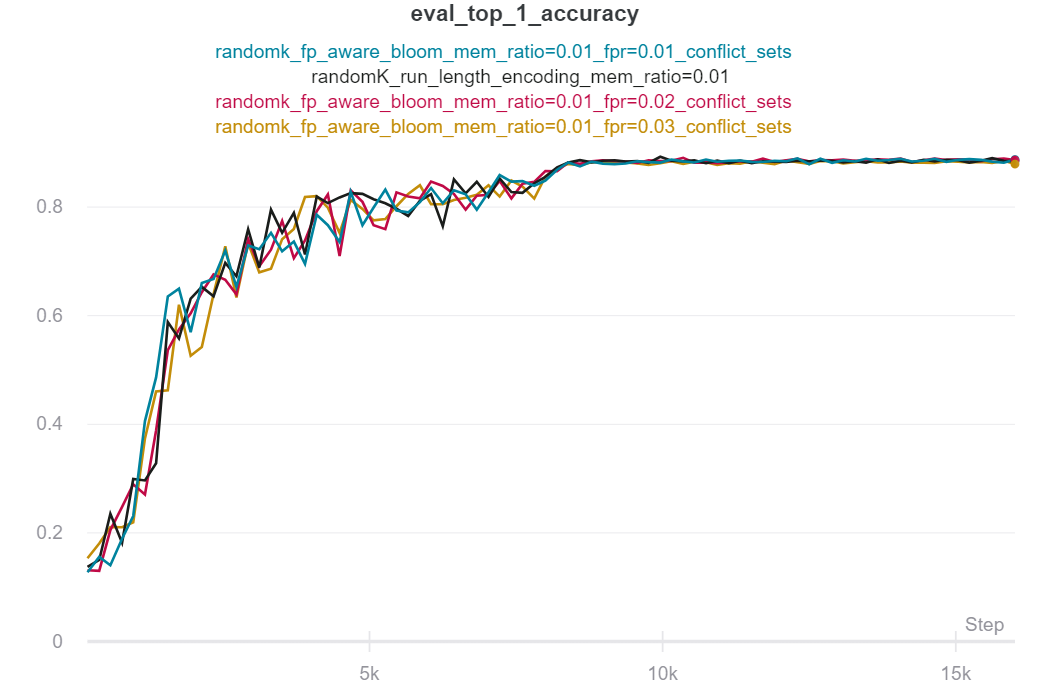
\includegraphics[width=1\textwidth]{thesis/figures/randomk-bloom.png}
    \caption{Resnet20, False-Positive-Aware Bloom Filter Compression}
    \label{randomk-bloom}
    \end{figure}
    
    \vspace{1cm}

    Notice that, this time, as we gradually increase the FPR we do not observe a degradation of the accuracy with respect to the baseline.
    Remember that, the False Positive Aware Compressor is a hybrid method that, under the absence of false positives, operates exactly like the underlying sparsification method. 
    However, when false positives start to occur, it starts to behave more and more like Random-r.
    Here, we use Random-r as our underlying compression method, so the occurrence of false positives will not have an effect.
    
    \vspace{1cm}

    \begin{table}[h!]
    \footnotesize
     \centering
    \begin{tabular}{ |p{3cm}||p{1cm}|p{1cm}|p{2cm}|p{1.6cm}|p{1.6cm}|p{1.3cm}|p{1.5cm}|}
    \hline
    \multicolumn{8}{|c|}{\textbf{\footnotesize Resnet20, compress\_ratio=0.01, Random-r, memory\_compensation}} \\
    \hline
    \rule{0pt}{3ex}
    	Method & Policy & FPR  &Initial-Bits &Final-Bits &Final/Initial & PER & Accuracy\\
    \hline
    \rule{0pt}{3ex}
    \multirow{4}{*}{\textbf{Fp-Aware Bloom}}
    & CS   &0.01     &   28832969 &   2803400 &    9.723\%  &18.83\%   &88.76\%\\
    & CS   &0.02     &   28832969 &   2395944 &    8.31\%   &44.68\%   &88.66\%\\
    & CS   &0.03     &   28832969 &   2121168 &    7.357\%  &62.46\%   &87.92\%\\
    \hline
    \rule{0pt}{3ex}
    \textbf{RLE}    & - & - & 28832969 & 2681248 & 9.299\%  &0   &88.47\%\\
    \hline
    \end{tabular}
    \caption{Resnet20: FP Aware Bloom Filter Compression on Random-r}
    Initial-Bits and Final-Bits refer to the indices and not the whole message. 
    \label{table:5}
    \end{table}
    %%%%%%%%%%%%%%%%%%%%%%%%%%%%%%%%%%%%%%%%%%%%%%%%%%%%%%%%%%%%%%%%%%%%%%%%%%%%%%%


    \newpage
    \section{Values Compression}
    
    In figures \ref{resnet_val_approx} and \ref{vgg_val_approx}, we provide the results of the values approximation approach for ResNet20 and VGG16. 
    They were both trained on the cifar10 dataset using some of the curve fitting techniques discussed in a previous section.
    Note that, we apply this method only for the convolutional layers of each model since those have a significantly large size that we need to reduce.
    
    %%%%%%%%%%%%%%%%%%%%%%%%%%%%%% RESNET20 %%%%%%%%%%%%%%%%%%%%%%%%%%%%%%%%%%%%%%%%%%%%
    \begin{figure}[h]
    \centering
    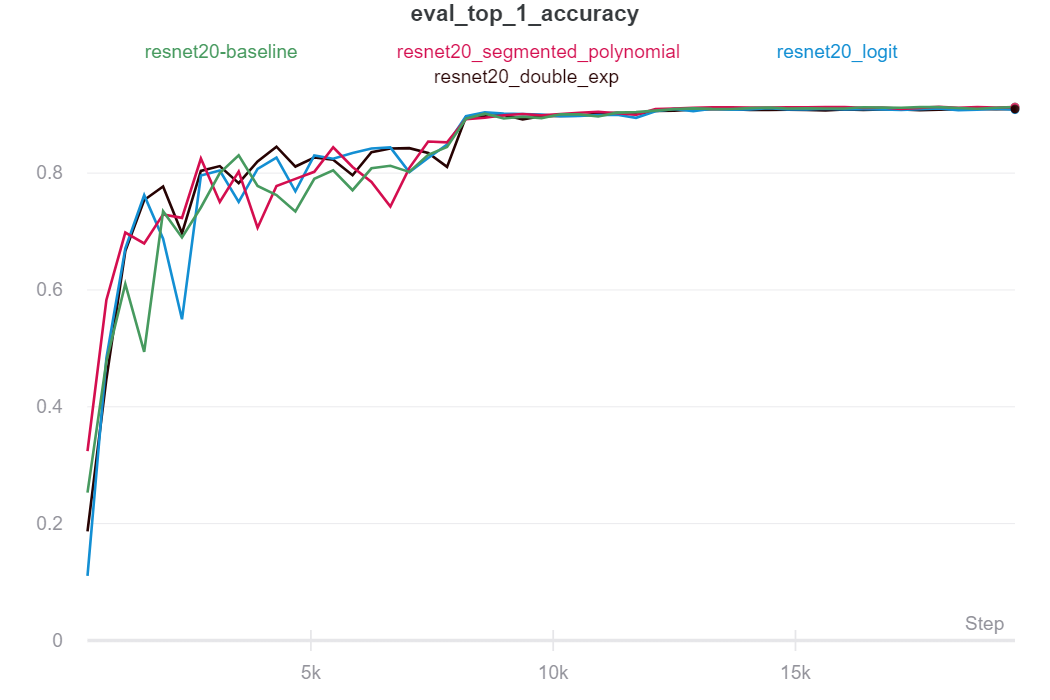
\includegraphics[width=1\textwidth]{thesis/figures/resnet-values-approx.png}
    \caption{Resnet20, Values Approximation}
    \label{resnet_val_approx}
    \end{figure}
    
    % \vspace{1cm}
    We observe that, ResNet20 reaches the baseline's accuracy in all cases, however, not all curve fitting methods provide equally good approximations.
    This was demonstrated in the figures of the "Fitting the tensor values" section where we could see that depending on the fitting technique the quality of the curves either increased or decreased.
    More specifically, we have observed that fitting segments of the tensor values using polynomial functions behaved better in terms of RMSE compared to the other approaches.
    
    \vspace{1cm}

    \begin{table}[h!]
    \footnotesize
     \centering
    \begin{tabular}{ |p{3cm}||p{3cm}|p{1.5cm}|}
    \hline
    \multicolumn{4}{|c|}{\textbf{\footnotesize Resnet20, compress\_ratio=0.01}} \\
    \hline
    \rule{0pt}{3ex}
    	Method & Basis Functions  & Accuracy\\
    \hline
    \rule{0pt}{3ex}
    \multirow{4}{*}{\textbf{Values Approx.}}
    & Logits       &90.85\%\\
    & Double Exp.  &90.97\%\\
    & Segm. Pol.   &91.29\%\\
    \hline
    \rule{0pt}{3ex}
    \textbf{No Compression} & -   &91.32\%\\
    \hline
    \end{tabular}
    \caption{Resnet20: Values Approximation}
    \label{table:6}
    \end{table}
    
    %%%%%%%%%%%%%%%%%%%%%%%%%%%%%%%%%%%%%%%%%%%%%%%%%%%%%%%%%%%%%%%%%%%%%%%%%%%%%%%

    
    %%%%%%%%%%%%%%%%%%%%%%%%%%%%%% VGG16 %%%%%%%%%%%%%%%%%%%%%%%%%%%%%%%%%%%%%%%%%%%%
    \begin{figure}[h]
    \centering
    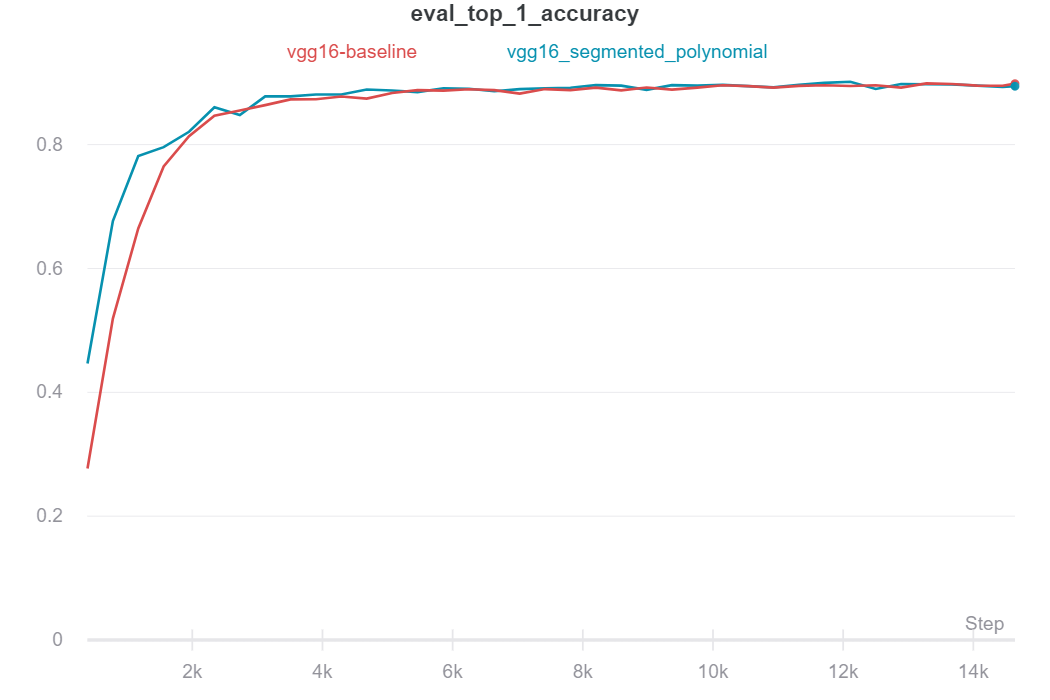
\includegraphics[width=1\textwidth]{thesis/figures/vgg-values-approx.png}
    \caption{VGG16, Values Approximation}
    \label{vgg_val_approx}
    \end{figure}

    \vspace{2cm}
    \newline
    VGG16's gradients are large in size and thus, fitting them with such numerical curve fitting methods was somewhat challenging.
    Training could halt at any point due to matrices being non-invertible, so for this model we chose to apply only the approach where we fit segments of the curve using polynomials. 
    This is a generally more flexible approach and by carefully selecting the segments offline we could manage to avoid those kind of errors completely.
    
    
    \vspace{1cm}

    \begin{table}[h!]
    \footnotesize
     \centering
    \begin{tabular}{ |p{3cm}||p{3cm}|p{1.5cm}|}
    \hline
    \multicolumn{3}{|c|}{\textbf{\footnotesize VGG16, compress\_ratio=0.01}} \\
    \hline
    \rule{0pt}{3ex}
    	Method & Basis Functions  & Accuracy\\
    \hline
    \rule{0pt}{3ex}
    \multirow{1}{*}{\textbf{Values Approx.}}
    & Segm. Pol. &89.43\%\\
    \hline
    \rule{0pt}{3ex}
    \textbf{No Compression} & - &89.85\%\\
    \hline
    \end{tabular}
    \caption{VGG16: Values Approximation}
    \label{table:6}
    \end{table}
    
    \vspace{5cm}

    %%%%%%%%%%%%%%%%%%%%%%%%%%%%%%%%%%%%%%%%%%%%%%%%%%%%%%%%%%%%%%%%%%%%%%%%%%%%%%%
    
    
    \section{TopK Values Compression}

    \begin{figure}[h]
    \centering
    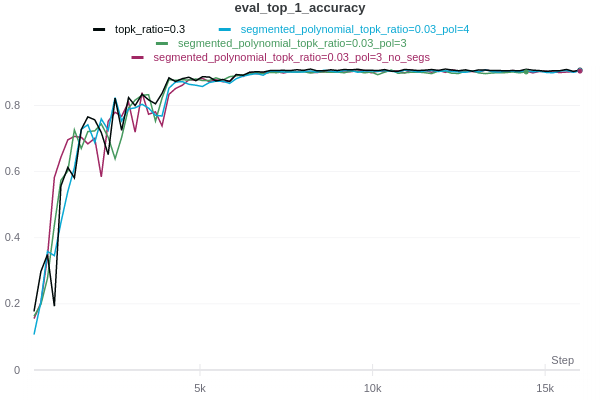
\includegraphics[width=1\textwidth]{thesis/figures/segmented_pol_topk.png}
    \caption{Resnet20, Topk Values Approximation}
    \label{resnet_val_approx}
    \end{figure}

    % \begin{table}[h!]
    % \footnotesize
    %  \centering
    % \begin{tabular}{ |p{3cm}||p{3cm}|p{1.3cm}|p{1.5cm}|}
    % \hline
    % \multicolumn{4}{|c|}{\textbf{\footnotesize Resnet20, compress\_ratio=0.3}} \\
    % \hline
    % \rule{0pt}{3ex}
    % 	Method & Basis Functions & RMSE & Accuracy\\
    % \hline
    % \rule{0pt}{3ex}
    % \multirow{4}{*}{\textbf{Values Approx.}}
    % & Logits      &-\%   &90.85\%\\
    % & Double Exp. &-\%   &90.97\%\\
    % & Segm. Pol.  &-\%   &91.29\%\\
    % \hline
    % \rule{0pt}{3ex}
    % \textbf{No Compression} & -   &0   &91.32\%\\
    % \hline
    % \end{tabular}
    % \caption{Resnet20: Values Approximation}
    % \label{table:6}
    % \end{table}
    
    \begin{table}[h!]
    \footnotesize
     \centering
    \begin{tabular}{ |p{3cm}||p{1cm}|p{1cm}|p{2cm}|p{1.6cm}|p{1.6cm}|p{1.3cm}|p{1.5cm}|}
    \hline
    \multicolumn{8}{|c|}{\textbf{\footnotesize Resnet20, compress\_ratio=0.3, Top-r, memory\_compensation}} \\
    \hline
    \rule{0pt}{3ex}
    	Method & Pol.D & Segs & Initial-Bits &Final-Bits &Final/Initial & RMSE & Accuracy\\
    \hline
    \rule{0pt}{3ex}
    \textbf{Pol.}       & 3 &  19 &  2569632 & 3648   &    0.141\%  &0.0423\%   &90.45\%\\
    \textbf{ Segm. Pol.} & 3 &  37 &  2569632 & 7104   &    0.276\%   &0.0301\%   &90.57\%\\
    \textbf{ Segm. Pol.} & 4 &  37 &  2569632 & 9472   &    0.368\%  &0.0177\%  &90.59\%\\
    \hline
    \rule{0pt}{3ex}
    \textbf{Baseline}   & - &  -  &  2569632 & 2569632 & 100\%  &0  &90.77\%\\
    \hline
    \end{tabular}
    \caption{Resnet20: Topk values approximation}
    'Pol.D' stands for the degree of polynomials used whereas 'Segs' is the total number of curve segments for all those gradients of one training step that correspond to convolutional layers.
    "Baseline" is the top-r sparsification method without any additional compression of the sparsified values. We use float variables of 32 bits to store each of those values.
    Final-Bits and Initial-Bits do not include the bits needed for sending the indices.
    They refer to the bits needed to communicate the "coefficients" or "values"  for all the gradients that correspond to convolutional layers for one training step with or without compression, respectively. We use 32-bit float variables to store the values without the values approximation compression while we use 64-bit float variables to store the coefficients when we use this compression method.
    Note that, these numbers are fixed throughout all the different training steps, thus we measure them only for one step in order to compute our gain-ratio (Final/Initial).
    Segm. Pol. refers to the method where we fit segments of the sparsified tensor values using polynomials.
    The number of segments is fixed for each gradient (here we choose 1 or 2) depending on its size.
    Pol. refers to the method where we fit all the sparsified tensor values using only one curve (no segments).
    Generally, as we reduce the number of segments, as well as the polynomial degree, we also reduce the Final-Bits even further. RMSE is computed by averaging all the RMSEs of the convolutional layer gradient fittings of one training step.
    
    \label{table:5}
    \end{table}
    
    
